\documentclass[10pt]{article}
\usepackage[utf8]{inputenc}
\usepackage{listings}
\usepackage{float}
\usepackage{graphicx}
\usepackage{fullpage}
\usepackage{caption}
\usepackage{subcaption}
\usepackage{amsmath}

%\renewcommand{\thesubsection}{\arabic{subsection}}
\renewcommand{\thesubsubsection}{\alph{subsubsection}}

\title{Pattern Recognition Practical 3}
\author{Group 24: \and Maikel Withagen (s1867733) \and Steven Bosch (s1861948)}
\date{\today}
\lstset{
frame=single, 
numbers=left, 
breaklines=true, 
language=Matlab,
basicstyle=\small, 
title=\lstname
}

\renewcommand{\thesection}{Assignment \arabic{section}}
\renewcommand{\thesubsection}{\arabic{subsection}}
\begin{document}

\maketitle

\section{Classification error, hit/false alarm rates, ROC curve, discriminability}
\subsection{}
Figure \ref{fig1.1} shows the ROC-curves we acquired using the code given in the listing for assignment 1.1 in the appendix. The figure shows that the higher the difference between the means of the two distributions is (i.e. the further away the distributions are from each other), the higher the number of hits is per number of fals alarms. This means that classification will go better when distributions are farther away from each other, which is of intuitively comprehensable as well.

\begin{figure}[H]
 \centering
 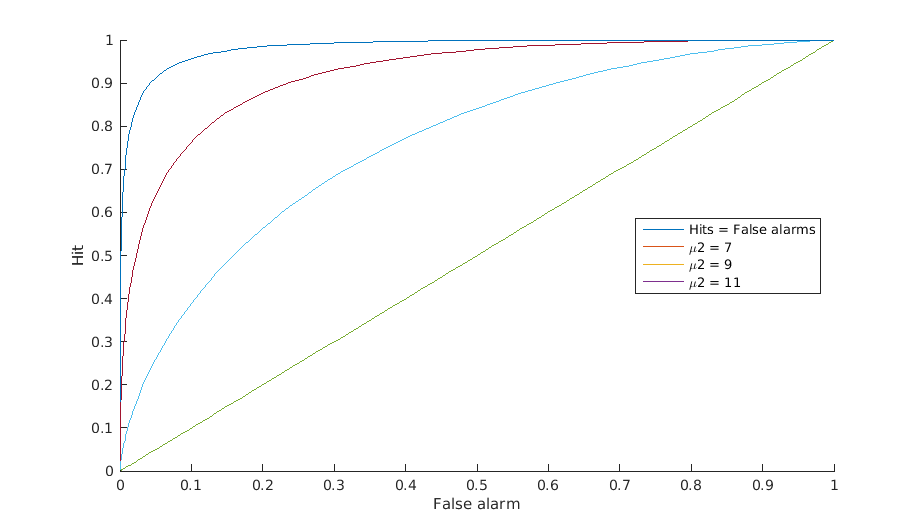
\includegraphics[width=\textwidth]{assign1_1.png}
 \caption{ROC-curves for $\mu_2={7, 9, 11}$ and the hits $=$ false alarms marker line.}
 \label{fig1.1}
\end{figure}

\subsection{}
Figure \ref{fig1.2} shows the point $(fa, h)$ of the two given binary vectors plotted in the plot computed in assignment 1.1. The listing for assignment 1.2 in the appendix gives the code used to compute this point and to compute the ROC-curve with the associated discriminability value $d'$. Trial and error yielded a ROC-curve with $d' \approx 1.5$ (this is an approximation, the exact value is a decimal value that is time-consuming to find by trial and error). We computed this using $\sigma_{1,2} = 1$, which yields $\mu_2-\mu_1 = 1.5$ for the found discriminability value. Note that the code in the listing gives $\sigma = 2$, which means $\mu_2-\mu_1 = 3$, since $d' = \frac{\mu_2-\mu_1}{\sigma}$. So as long as the discriminability valueb between two distributions is the same, the sigma does not matter for classification. 

\begin{figure}[H]
 \centering
 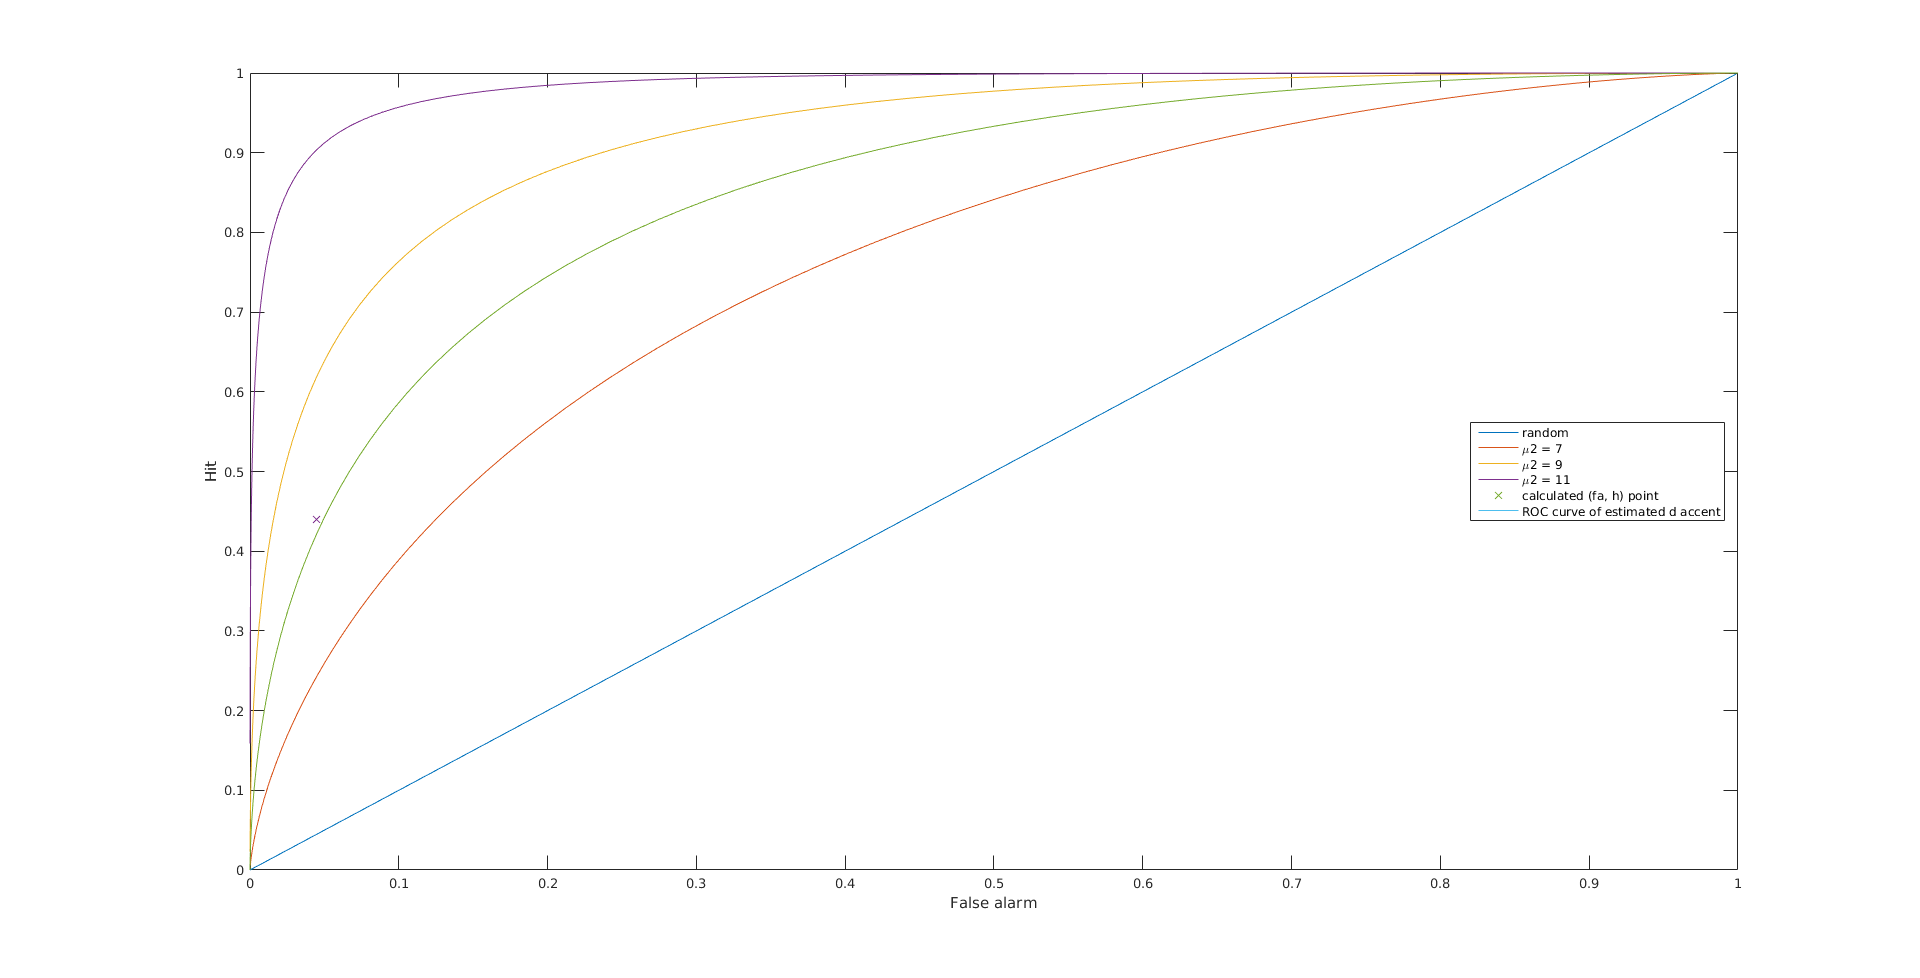
\includegraphics[width=\textwidth]{assign1_2b.png}
 \caption{Plot of the $(fa, h)$ point, the ROC-curves for $\mu_2={7, 9, 11}$, the hits $=$ false alarms marker line, and the ROC-curve with $d'=1.5$.}
 \label{fig1.2}
\end{figure}

\section{K-nearest neighbor classification}
\subsection{}
Our implementation of the KNN-function is the following:
\lstinputlisting{../Code/assign2_1}

\subsection{}
For $k=1$ this yields the following Voronoi diagram:
\begin{figure}[H]
 \centering
 \includegraphics[width=\textwidth]{assign2_1a.png}
 \caption{Voronoi diagram of the data set using KNN (for $k=1$)}
 \label{fig2.1a}
\end{figure}

For $k=3$ this yields the following Voronoi diagram:
\begin{figure}[H]
 \centering
 \includegraphics[width=\textwidth]{assign2_1b.png}
 \caption{Voronoi diagram of the data set using KNN (for $k=3$)}
 \label{fig2.1b}
\end{figure}

For $k=5$ this yields the following Voronoi diagram:
\begin{figure}[H]
 \centering
 \includegraphics[width=\textwidth]{assign2_1c.png}
 \caption{Voronoi diagram of the data set using KNN (for $k=5$)}
 \label{fig2.1c}
\end{figure}

For $k=7$ this yields the following Voronoi diagram:
\begin{figure}[H]
 \centering
 \includegraphics[width=\textwidth]{assign2_1d.png}
 \caption{Voronoi diagram of the data set using KNN (for $k=7$)}
 \label{fi2.1d}
\end{figure}

\subsection{}

\section{Parzen windows, posterior probabilities}

\section*{Appendix}
\lstinputlisting{../Code/assign1_1.m}
\lstinputlisting{../Code/assign1_2.m}

\end{document}
